\documentclass[fleqn, 12pt]{article}

\usepackage[utf8]{inputenc}
\usepackage[bulgarian]{babel}
\usepackage{amsmath}
\usepackage{amssymb}
\usepackage{booktabs}
\usepackage{fancyhdr}
\usepackage{amsthm}
\usepackage{graphicx}


\newtheorem{definition}{Дефиниция}[subsection]
\newtheorem{theorem}{Tеорема}[subsection]
\theoremstyle{definition}
\newtheorem{example}{Пример}[subsection]


\title{Физика \\ Формули и теореми}
\author{Exonaut}

\pagestyle{fancy}
\fancyhf{}
\lhead{\rightmark}
\rhead{\thepage}
\cfoot{}
\renewcommand{\headrulewidth}{0pt}

\begin{document}
\maketitle
\pagenumbering{gobble}
\newpage
\pagenumbering{arabic}

\tableofcontents

\newpage
\section{Лекция 1: Кинематика}

\subsection{Теория}

\begin{itemize}
\item \textbf{Материална точка (МТ)} - Точка с пренебрежителни размери и форма
\item \textbf{Отправно тяло (ОТ)} - Тяло, спрямо което отчитаме движението 
\item \textbf{Отправна система (ОС)} - ОT, кординатна система и часовник
\item \textbf{Радиус вектор} - Вектор от началото на ОС до точка. Бележи се с $\vec{r}(t)$
\item \textbf{Траектория} - Линия, описвана от МТ при джиението ѝ 
\item \textbf{Път} - Дължината на траекторията до края 
\item \textbf{Преместване} - Вектор от началото до края 
\item \textbf{Праволинейно движение} - Движение по едно направление
\end{itemize}

\begin{center}
\begin{tabular}{ |c|c|c|}
\hline
\textbf{Понятие} &\textbf{Означение} & \textbf{Мерни единици}\\
\hline
Средна скорост & $V(t)$ & Основна - $\frac{m}{s}$, Ползва се и $\frac{km}{h}$\\
\hline
Моментна скорост & $V(t)$ & Основна - $\frac{m}{s}$, Ползва се и $\frac{km}{h}$\\
\hline
Средно ускорение & $a(t)$ & $\frac{m}{s^2}$\\
\hline
Моментно ускорение & $a(t)$ & $\frac{m}{s^2}$\\
\hline
\end{tabular}
\end{center}

\newpage
\subsection{Формули}

\begin{itemize}
\item Радиус вектор (x,y,z - кординати в тримерното пространство)
$$r= \sqrt{x^2 + y^2 + z^2}$$
\item Средна скорост
$$\vec{V_{\text{ср}}} = \frac{\Delta \vec{r}}{\Delta t}$$
\item Момента скорост
$$V = \frac{d\vec{r}}{dt}$$
\item Средно ускорение
$$\vec{a_{\text{ср}}} = \frac{\Delta \vec{V}}{\Delta t} $$
\item Моменто ускорение
$$a = \frac{d\vec{V}}{dt} = \frac{d^2 \vec{r}}{dt^2}$$
\item Закон за скоростта ($V_0$ - начална скорост)
$$V = V_0 + at$$
\item Закон за движение ($x_0$ - начален път,$V_0$ - начална скорост)
$$x = x_0 + V_0t \pm \frac{at^2}{2}$$
\item Скорост при неправолинейно движение
$$V_x = \frac{dx}{dt} \quad V_y = \frac{dy}{dt} \quad V_z = \frac{dz}{dt} \quad V = \sqrt{V_x^2 + V_y^2 + V_z^2}$$
\item Ускорение при неправолинейно движение
$$a_x = \frac{dV_x}{dt} \quad a_y = \frac{dV_y}{dt} \quad a_z = \frac{dV_z}{dt}  \quad a = \sqrt{a_x^2 + a_y^2 + a_z^2}$$
\item Скорост спрямо ъгъл ($V_0$ - начална скорост, $\alpha$ - ъгъл)
$$V_x = V_0 \cos \alpha \qquad V_y = V_0 \sin \alpha$$
\item Закон за движение при падане
$$y = y_0 + V_{0y} - \frac{gt^2}{2} $$
\item Други формули
$$x = x_0 + Vt \qquad V = V_0 \pm at \qquad \tan \alpha = \frac{V_y}{V_x}$$
\item Превръщане от $\frac{m}{s}$ в $\frac{km}{h}$ 
$$1 \frac{m}{s} = 3.6 \frac{km}{h}$$
\end{itemize}

\newpage
\section{Лекция 2: Динамика на материална точка}

\subsection{Теория}

\begin{itemize}
\item \textbf{I-ви принцип на Нютон}: Всяко тяло запазва състоянието си на покой или на праволинейно
равномерно движение, докато външно въздействие не го изведе от това състояние.
\item \textbf{III-ви принцип на Нютон}: Силите на взаимодействие между две тела са равни
по големина и противоположни по посока.
\item \textbf{Закон на Нютон за гравитацията}: Между всеки две материални точки
действа сила на привличане, която е правопропорционална на произведението на
масите им и обратно пропорционална на квадрата на разстоянието между тях.
\item Консервативни сили - сили, чиято работа не зависи от вида на траекторията, а се определя само от началното и крайното положение. Пример: гравитационната сила, силата на тежестта, еластичните сили, електростатичните сили
\item \textbf{Закона за запазване на енергията}: В една затворена механична система, в която
действат само консервативни сили, пълната механична енергия е константа.
\end{itemize}

\begin{center}
\begin{tabular}{ |c|c|c|}
\hline
\textbf{Понятие} &\textbf{Означение} & \textbf{Мерни единици}\\
\hline
Маса & $m$ & kg \\
\hline
Сила & $\vec{F}$ & N (Нютон) \\
\hline 
Импулс & $\vec{p}$ & $\frac{kg \cdot m}{s}$ \\
\hline
Сила на тежестта & $G$ & N\\
\hline
Реакция на опората & $N$ & N \\
\hline
Сила на триене & $f$ & N \\
\hline
Работа & $A$ & J (Джаул)\\
\hline
Мощност & $P$ & W (Ват)\\
\hline
Кинетична енергия & $E_k$ & J \\
\hline
Потенциална енергия & $E_p$ & J \\
\hline
\end{tabular}
\end{center}

\newpage
\subsection{Формули}
\begin{itemize}
\item Импулс
$$\vec{p} = m \vec{V}$$
\item II-ри закон на Нютон
$$\vec{F} = \frac{d \vec{p}}{dt} \qquad F= ma$$
\item Гравитационна сила
$$F = \gamma \frac{m_1 m_2}{r^2}$$
\item Сила на тежестта (М - маса на земята, R - разстояние до центъра на земята)
$$G = \gamma \frac{mM}{R^2} \qquad G = mg$$
\item Реакция на опората
$$N = mg$$
\item Сила на триене
$$f = kN \qquad k(\text{коефициент на триене}$$
\item Закон за запазване на импулса (ЗЗИ) 
$$\vec{p} = const$$
\item Работа ($\alpha$ - ъгъл между силата и преместването, $F_x, F_y, F_z$ - компоненти на силата, $dx,dy,dz$ - копоненти на преместването. $\Delta r$ - преместване от един радиус вектор в друг радиус вектор)
$$dA = \vec{F} d\vec{r} = F dr \cos \alpha \qquad dA = F_x dx + F_y dy + F_z dz \qquad A = F \Delta r \cos \alpha$$
\item Мощност 
$$P = \frac{dA}{dt}$$
\item Кинетична енергия 
$$E_k = \frac{mV^2}{2}$$
\item Потенциална енергия (h - височина над земята)
$$E_p = mgh$$
\item Пълна механична енергия на система
$$E = E_k + E_p$$
\item Закон за запазване на енергията (ЗЗЕ)
$$E_1 = E_2 \Leftrightarrow E_{k1} + E_{p1} = E_{k2} + E_{p2}$$
\item Галилееви трансформации \\
Две системи K(неподвижна) и K'(движи се праволинейно равномерно със скорост $\vec{v_0}$) \\
Разположение на кординати: K: x,y,z; K': x',y',z' \\
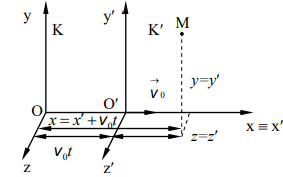
\includegraphics{Pics/physics/lec2-1.png} \\
Aко $v << c$
$$x = x' + V_0t \qquad y = y' \qquad z = z' \qquad t = t'$$
При $v \to c \implies$ Препобразувания на Лоренц
Връзка на скоростите в двете системи
$$V_x = V'_x + V_0 \qquad V_y = V'_y  \qquad  V_z = V'_z \implies \vec{V} = \vec{V'} + \vec{V_0}$$
$$\vec{a} = \vec{a'} \qquad \vec{F} = \vec{F'}$$
\end{itemize} 
\newpage
\subsection{Константи}

\begin{center}
\begin{tabular}{ |c|c|c|}
\hline
\textbf{Означение} & \textbf{Наименование}&\textbf{Стойност}\\
\hline
$\gamma$ & гравитационна константа & $6.67 \cdot 10^{-11} \frac{N m^2}{kg^2}$ \\
\hline
$g$ & земно ускорение & $\approx 9.8 \frac{m}{s^2}$ \\
\hline
\end{tabular}
\end{center}

\newpage
\section{Лекция 3: Механика на идеално твърдо тяло}

\subsection{Теория}

\begin{center}
\begin{tabular}{ |c|c|c|}
\hline
\textbf{Понятие} &\textbf{Означение} & \textbf{Мерни единици}\\
\hline
Ъгъл на завъртане & $\varphi $ & \\
\hline
Средна ъгълова скорост & $\omega_{\text{ср}} (t)$ & $\frac{rad}{s}$\\
\hline
Моментна ъгълова скорост & $\omega (t)$ & $\frac{rad}{s}$\\
\hline
Средно ъгълово ускорение & $\alpha_{\text{ср}} (t)$ & $\frac{rad}{s^2}$\\
\hline
Моментно ъгълово ускорение & $\alpha (t)$ & $\frac{rad}{s^2}$\\
\hline
Период & $T$ & $s$ \\
\hline 
Честота & $\nu$ & $\text{Hz} = \frac{1}{s}$ (Херц)\\
\hline 
Момент на силата & $ \vec{M} $ & $Nm$\\
\hline 
Момент на импулса & $ \vec{L} $ & $\frac{kg \cdot m^2}{s}$\\
\hline
Инерчен момент & $I$ & $kg \cdot m^2$\\
\hline
\end{tabular}
\end{center}
\newpage
\subsection{Формули}

\begin{itemize}
\item Средна ъглова скорост
$$\vec{\omega_{\text{ср}}} = \frac{\Delta \vec{\varphi}}{\Delta t}$$
\item Моментна ъглова скорост
$$\vec{\omega} = \frac{d\vec{\varphi}}{dt}$$
\item Средно ъглово ускорение
$$\vec{\alpha_{\text{ср}}} = \frac{\Delta \vec{\omega}}{\Delta t}$$
\item Моментно ъглово ускорение
$$\vec{\alpha} = \frac{d\vec{\omega}}{dt} = \frac{d^2 \vec{\varphi}}{d^2 t}$$
\item Период, честота и връзка между тях
$$\nu \qquad T = \frac{1}{\nu} \qquad T\nu = 1$$
\item Скорост изразена чрез честота и период
$$\omega = \frac{\Delta \varphi}{\Delta t} = \frac{2 \pi }{T} = 2 \pi \nu$$
\item Закон за ъглова скорост($\omega_0$ - начална ъглова скорост)
$$\omega = \omega_0 + \alpha t$$
\item Закон за ъглово движение ($\varphi_0$ - начален път, $\omega_0$ - начална ъглова скорост)
$$\varphi = \varphi_0 + \omega_0 + \frac{\alpha t^2}{2}$$
\item Изминат път изразен чрез ъглъл на завъртане
$$S = R \Delta \varphi $$
\item Скорост изразена чрез ъглова скорост
$$V = R \omega$$
\item Тангенциално ускорение изразено чрез ъглово ускорение
$$a_t = R \alpha$$
\item Нормално ускорение изразено чрез ъглова скорост
$$a_n = \frac{V^2}{R} = \omega^2 R$$
\item Mомент на силата
$$\vec{M} = \vec{r} \times \vec{F}$$
\item Момент на импулса 
$$\vec{L} = \vec{r} \times \vec{p} = \vec{r} \times m \vec{V} \qquad L = \sum_{i=1} ^m \vec{L_i} = \sum_{i=1} ^m \left( \vec{r_i} \times \vec{p_i}\right) (\text{за система от n точки})$$
\item Oсновно уравнение на динамиката на въртеливи движение
$$\vec{M} = \frac{d \vec{L}}{dt}$$
\item Закон за запазване на момент на импулса
$$\frac{d \vec{L}}{dt} = 0 \qquad \vec{L} = const$$
\item Инерчен момент
$$I = mr^2, I = \sum_{i=1} ^m m_i r_i ^2$$
\item Момент на импулса (2)
$$L = I \omega$$
\item Oсновно уравнение (2)
$$M = I \alpha$$
\item Кинетична енергия 
$$E_k = \frac{I \omega^2}{2}$$
\item Работа
$$dA = M d\varphi$$
\end{itemize}

\newpage
\section{Лекция 4: Термодинамика}

\subsection{Теория}

\begin{itemize}
\item \textbf{Термодинамична система} - наричаме тяло или система от тела,
съставени от голям брой частици. Телата взаимодействат и обменят енергия както
помежду си, така и с външната среда.
\item \textbf{Термодинамично равновесие} - ако параметрите не променят стойностите си и в системата няма потоци. 
\item \textbf{Идеален газ} - газ на който собственият обем на молекулите се пренебрегва и между молекулите няма сили на взаимодействие.
\item Видове процеси
\begin{itemize}
\item Изотермен - температурата e постоянна.
\item Изобарен – налягането е постоянно.
\item Изохорен - обемът е постоянен.
\item Адиабатен - няма топлообмен с околната среда.
\end{itemize}
\item \textbf{I-ви принцип на термодинамиката} - Aко на една
термодинамична система предадем определено количество топлина
$Q $, то се изразходва за изменение на вътрешната енергия
$\Delta U$ и за извършване на работа $A$.
\item Видове процеси
\begin{itemize}
\item \textbf{Равновесен процес} - процес, при който термодинамичната система 
преминава през последователност от равновесни състояния. Само безкрайно бавни процеси могат да се разглеждат като равновесни.
\item \textbf{Обратим процес} - протича в права и обратна посока през едни и
същи междинни положения.
\item \textbf{Кръгов процес (цикъл)} - процес, при който
термодинамичната система се връща в началното си
положение.
\end{itemize}
\item \textbf{Цикъл на Карно} - цикъл с 2 изотермни и 2 адиабатни процеса
\item II-ри принцип на термодинамиката 
\begin{itemize}
\item Формулировка на Клаузиус (1850г.): \textbf{Не е възможен термодинамичен процес,
единственият краен резултат от който да е предаване на количество топлина от
термодинамична система с по-ниска температура на термодинамична система с по-висока температура.}
\item Формулировка на Келвин (1851г.): \textbf{Не е възможен кръгов процес,
единственият краен резултат от който е извършване на работа за сметка на охлаждане на една термодинамична система.}
\end{itemize}
\end{itemize}

\begin{center}
\begin{tabular}{ |c|c|c|}
\hline
\textbf{Понятие} &\textbf{Означение} & \textbf{Мерни единици}\\
\hline
Обем & $V$ & $m^3$ \\
\hline
Налягаме & $p$ & Pa (Паскал) $ = \frac{N}{m^2}$ \\
\hline
Температура & $t, \, T$& t - C (Целзий), T - K(Келвин) \\
\hline
Mаса на газа& $m$ & kg\\
\hline
Моларна маса & $M$ & $\frac{g}{mol}, \, \frac{kg}{mol}$\\
\hline
Брой молове & $\nu$ & mol\\
\hline
Количество топлина & $Q$ & J \\
\hline
Вътрешна енергия & $U$ & J \\
\hline
Топлинен капацитет & $C$& $\frac{J}{kg \cdot K}$ \\
\hline
Моларен топлинен капацитет & $C_m$& $\frac{J}{kg \cdot K}$ \\
\hline
Топлинен капацитет при пост. обем & $C_V$& $\frac{J}{kg \cdot K}$ \\
\hline
Топлинен капацитет при пост. налягане& $C_p$& $\frac{J}{kg \cdot K}$ \\
\hline
Коефициент полезно действие (КПД)& $\eta$&  \% \\
\hline
\end{tabular}
\end{center}

\newpage
\subsection{Формули}

\begin{itemize}
\item Налягане(S - площ)
$$p = \frac{F}{S}$$
\item Връзка между температура в Целзий и Келвин
$$T = t + 273$$
\item Закон на Бойл-Мариот($T = const, N = const$, N - брой частици)
$$pV = const \qquad p_1 V_1 = p_2 V_2 \text{(за две състояния)}$$
\item Закон на Шарл ($V = const, N = const$)
$$\frac{p}{T} = const \qquad \frac{p_1}{T_1} = \frac{p_2}{T_2} \text{(за две състояния)}$$
\item Закон на Гей-Люсак($p = const, N = const$)
$$\frac{V}{T} = const \qquad \frac{V_1}{T_1} = \frac{V_2}{T_2} \text{(за две състояния)}$$
\item Закон на Далтон (Смес от няколко газа, $p_1, p_2,...$ - налягания на газовете в сместа (парциално налягане))
$$p = p_1 + p_2 + ... p_n$$
\item Уравнение за състоянието на идеален газ (Закон на Клапейрон - Менделеев)
$$pV = \nu R T$$
\item I-ви принцип на термодинамиката
$$Q = \Delta U + A \qquad \delta Q = dU + \delta A \Leftrightarrow \delta Q = dU + p dV\text{(за безкрайно малки измерения)} $$
\item Топлинен капацитет
$$C = \frac{Q}{m \Delta T}$$
\item Моларен топлинен капацитет
$$C_m = \frac{Q}{\nu \Delta T} \quad C_m = \frac{\delta Q}{dT} \quad C_m = \frac{dU + pdV}{dT}$$
\item Топлинен капацитет при постоянен обем
$$ dV = 0 \implies C_V = \frac{dU}{dT}$$
\item Топлинен капацитет при постоянно налягане
$$ dp = 0 \implies C_p =\frac{dU + pdV}{dT} = \frac{dU}{dT} +  p\frac{dV}{dT} = C_V + p\frac{dV}{dT} \left( p\frac{dV}{dT} = R \text{(ур-е на състоянието)} \right)$$
\item Изопроцеси и работа при тях
\begin{center}
\begin{tabular}{ |c|c|c|c|c| } 
\hline
Процес & Изобарен  & Изохорен & Изотермен & Адиабатен \\
\hline
Осн. зависимости & $V = V_0 \alpha T$ & $p = p_0 \alpha T$ & $pV = const$ & $pV^\gamma = const$ \\
\hline 
I-ви принцип на ТД  & $\delta Q = dU + \delta A$ & $\delta Q = dU$ & $\delta Q = \delta A$ & $dU = - \delta A$\\
\hline
Работа  & $A = p(V_2 - V_1)$ & A = 0 & $A = \nu RT \ln {\frac{V_2}{V_1}}$ & $A = \nu C_V (T_1 - T_2)$\\
\hline
\end{tabular}
\end{center}
\item Уравнение на Майер
$$C_p = C_V + R$$
\item Коефициент полезно действие (КПД)
$$\eta = \frac{A}{Q}$$
\item КПД на цикъл на Карно
$$\eta = 1 - \frac{T_2}{T_1}$$

\end{itemize}

\newpage
\subsection{Константи}

\begin{center}
\begin{tabular}{ |c|c|c|}
\hline
\textbf{Означение} & \textbf{Наименование}&\textbf{Стойност}\\
\hline
$\alpha$ & коефициент на температурата & $\frac{1}{273} K^{-1}$\\
\hline
$N_A$ & Число на Авогадро & $6.022 \cdot 10^{-23} mol^{-1}$\\
\hline
R & Универсална газова константа & $8.314 \frac{J}{mol \cdot K}$\\
\hline
\end{tabular}
\end{center}

\newpage
\section{Лекция 5: Молекулна физика}

\subsection{Формули}
\begin{itemize}
\item Основно уравнение на молекулно-кинетичната теория (N - брой молекули, $\overline{v_i}$ - средна скорост на една молекула)
$$pV = \frac{1}{3} Nm \overline{v_i ^2}$$
\item Средна кинетична енергия на молекулите
$$\overline{E_k} = \frac{m \overline{v_i ^2}}{2}$$
\item Основно уравнение на молекулно-кинетичната теория(2)
$$pV = \frac{2}{3} N\overline{E_k}$$
\item Основно уравнение на молекулно-кинетичната теория при $N = N_A$
$$pV = \frac{3}{2} k T$$
\item Вътрешна енергия на идеален газ
$$U = \sum_{i=1} ^N E_{ki} = N \overline{E_k}$$
\item Представяне на налягане чрез температура(n - концентрация, N - брой молекули)
$$p = nkT, \qquad n = \frac{N}{V}$$
\item Функция на разпределение на Максуел
$$f(v) = 4 \pi \left( \frac{m}{2 \pi k T}\right)^{\frac{3}{2}} \cdot v^2 \cdot \exp \left(- \frac{m v^2}{2 k T} \right)$$
\item Разпределение на Болцман($n_0$ - концентрация при $E_p = 0$)
$$n = n_0 \cdot \exp \left( - \frac{E_p}{kT}\right)$$
\end{itemize}

\newpage
\subsection{Константи}

\begin{center}
\begin{tabular}{ |c|c|c|}
\hline
\textbf{Означение} & \textbf{Наименование}&\textbf{Стойност}\\
\hline
k & Константа на Болцман & $k = \frac{R}{N_A} = 1.38 \cdot 10^{-23} \frac{J}{K}$ \\
\hline
\end{tabular}
\end{center}

\newpage
\section{Лекция 6: Електростатика}

\subsection{Теория}

\begin{itemize}
\item Интензитетът е силова характеристика на полето. 
\item \textbf{Принцип на суперпозицията}: всеки заряд създава електрично поле независимо от наличието на други заряди. 
\item \textbf{Еднородно (хомогенно) поле}: интензитетът е един и същ за всяка точка от полето. 
\item \textbf{Силовии линии}: показват посоката на интензитета; излизат от + и влизат в -; по-силно поле се изобразява като силовите линии се чертаят по нагъсто
\item \textbf{Закон на Гаус}: Потокът на интензитета през затворена повърност е раве на затворения в повърхността заряд разделен на $\varepsilon_0$
\item \textbf{Проводници}: провеждат ток, имат свободни електрони.
\item \textbf{Кондензатор}: система от два проводника, разделени от диелектрик, заредени с равни по големина и различни по знак заряди и с такава форма и разположение при която ел. поле е между проводниците. 
\item \textbf{Диелектрици (Изолатори)}: нямат свободни заряди.
\end{itemize}

\begin{center}
\begin{tabular}{ |c|c|c|}
\hline
\textbf{Понятие} &\textbf{Означение} & \textbf{Мерни единици}\\
\hline
Заряд& $q, Q, q_t$ (пробен заряд)& $C$ (Кулон) \\
\hline 
Относителна диел. проницаемост& $\varepsilon_r$& \\
\hline
Интензитет& $\vec{E}$ & $\frac{N}{C}$ \\
\hline
Поток на интензитета & $\Phi_E$ & ?? \\
\hline
Потенциална енергия & $W(r)$ & $J$ \\
\hline
Потенциал & $\varphi$ & $V$ (Волт)\\
\hline
Напрежение (Потенциална разлика) & $U$ & $V$\\
\hline
Капацитет на кондензатор & $C$ & $F$ (Фарад) \\
\hline
\end{tabular}
\end{center}

\newpage
\subsection{Формули}

\begin{itemize}
\item Закон на Кулон във вакуум
$$F = \frac{q_1q_2}{4\pi \varepsilon_0 r^2} \qquad
\text{По някога:}\, F = \frac{kq_1q_2}{r^2}, \ k = \frac{1}{4\pi \varepsilon_0}$$
\item Закон на Кулон във среда
$$F = \frac{q_1q_2}{4\pi \varepsilon_0 \varepsilon_r r^2} \qquad
\text{По някога:}\, F = \frac{kq_1q_2}{r^2}, \ k = \frac{1}{4\pi \varepsilon_0 \varepsilon_r}$$
\item Интензитет на поле 
$$\vec{E} = \frac{\vec{F}}{q_t} = \frac{q}{4\pi \varepsilon_0 r^2}$$
\item Поток на интензитета
$$d\Phi_E = E \cdot dS \cdot \cos \alpha \qquad \Phi_E = \int E \cdot dS \cdot \cos \alpha $$
\item Закон на Гаус
$$\Phi_E = \frac{q}{\varepsilon_0} \qquad \Phi_E = \frac{\sum q}{\varepsilon_0} \text{(повече от един заряд)}$$
\item Потенциална енергия
$$W(r) = \frac{qq_t}{4 \pi \varepsilon_0 r}$$
\item Работа на електростатично поле
$$ A = - \left(\frac{q q_t}{4 \pi \varepsilon_0 r_1} - \frac{q q_t}{4 \pi \varepsilon_0 r_2} \right)
\qquad 
A = -(W_2 - W_1)$$ 
\item Потенциал 
$$\varphi = \frac{W}{q_t} = \frac{q}{4 \pi \varepsilon_0 r}$$
\item Напрежение 
$$U = \varphi_1 - \varphi_2 \qquad U = \frac{A}{q_t}$$
\item Интензитет на поле
$$E_x = -\frac{d\varphi}{dx}$$
\item Капацитет на кондензатор (обща формула)
$$C = \frac{q}{U}$$
\item Капацитет на въздушен кондензатор (d -  разтояние между плочи, S - площ на плоча) 
$$C = \varepsilon_0 \frac{S}{d}$$
\item Капацитет на плосък кондензатор (d -  разтояние между плочи, S - площ на плоча) 
$$C = \varepsilon_0 \varepsilon_r \frac{S}{d}$$
\end{itemize}

\newpage
\subsection{Константи}

\begin{center}
\begin{tabular}{ |c|c|c|}
\hline
\textbf{Означение} & \textbf{Наименование}&\textbf{Стойност}\\
\hline
$e$ & Заряд на електрона & $e =  1.6 \cdot 10^{-19} C$ \\
\hline
$\varepsilon_0$ & Електрична константа & $\varepsilon_0 =  8.85 \cdot 10^{-12} \frac{C^2}{N \cdot m^2}$ \\
\hline
$k$ &  & $ k= \frac{1}{4\pi \varepsilon_0} = 9 \cdot 10^9 Nm^2$ \\
\hline
\end{tabular}
\end{center}

\newpage
\section{Лекция 7: Електричен ток}

\subsection{Теория}
\begin{itemize}
\item \textbf{Eлектродвижещо напрежение(ЕДН)}: работата на страничните сили за пренасяне на заряд срещу силите на електричното поле разделена на големината на пренесения заряд.
\end{itemize}

\begin{center}

\begin{tabular}{ |c|c|c|}
\hline
\textbf{Понятие} &\textbf{Означение} & \textbf{Мерни единици}\\
\hline
Електричен ток & $I$ & $А$ (Ампер)\\
\hline
Плътност на тока& $j$ & $\frac{A}{m^2}$\\
\hline
Eлектродвижещо напрежение(ЕДН) & $\varepsilon$ & $V$ (волт) \\
\hline
Съпротивление & $R$ & $\Omega$ (Ом) \\
\hline
Специфично съпротивление & $\rho$ & $\Omega \cdot m$ \\
\hline
\end{tabular}
\end{center}

\newpage
\subsection{Формули}
\begin{itemize}
\item Елетричен ток 
$$I = \frac{dq}{dt} \qquad I = \frac{q}{t} \text{(постоянен ток)}$$
\item Плътност на тока 
$$j = \frac{dI}{dS_{\perp}} \qquad j = \frac{I}{S} \text{(постоянен ток)} \qquad I = jS$$
\item Eлектродвижещо напрежение(ЕДН) 
$$\varepsilon = \frac{A_{\text{странични}}}{q}$$
\item Закон на Ом за част от верига (познато като "URI - URItarted")
$$R = \frac{U}{I} \implies U=RI \qquad I = \frac{U}{R}$$
\item Специфично съпротивление (l - дължина на провидника, S - напречно сечение)
$$R = \rho \frac{l}{S}$$
\item Закон на Ом за цялата верига (R - общо съпротивление на веригата, r - съпротивление на източника)
$$I = \frac{\varepsilon}{R + r}$$
\item Работа 
$$A = \int\limits_{t_1} ^{t_2} UI \ dt \qquad A = UIt \text{(постоянен ток)}$$
\item Мощност
$$P = UI = I^2R = \frac{U^2}{R}$$
\item Закон на Джаул-Ленц
$$Q = I^2Rdt = \frac{U^2}{R} dt \qquad Q = I^2Rt = \frac{U^2}{R}t $$
\item Последователно свързване на n консуматора
$$I = const \qquad U = \sum_{i=1} ^n U_i  \qquad R = \sum_{i=1} ^n R_i$$
\item Успоредно (паралелно) свързване на n консуматора 
$$I = \sum_{k=1} ^n I_k \qquad U = const \qquad \frac{1}{R} = \sum_{k=1} ^n \frac{1}{R_k}$$
\end{itemize}

\newpage
\section{Лекция 8: Магнетизъм}

\subsection{Теория}

\begin{itemize}
\item \textbf{Магнитни полета}: създават се от постоянни магнити или електричен ток
\item Магнит има два полюса: северен (N) и южен (S). Еднакви полюси се отблъскват, различните се привличат. 
\item \textbf{Правило на дясната ръка (за прав проводник)}: Палецът на дясната ръка сочи
посоката на тока, свитите пръсти сочат посоката на магнитната индукция. 
\item \textbf{Закон на Ампер}: Циркулацията по произволен затворен контур е равна на алгебричната сума от токовете пронизващи контура 
\item \textbf{Закон на Фарадей}: Явлението, при което в затворен проводников контур протича ток при промяна на магнитния поток през контура се нарича електромагнитна индукция.  
\item \textbf{Правило на Ленц}: Индуцираният ток има такава посока, че създаденото от него магнитно поле се противопоставя на измененията на външния магнитен поток.
\item \textbf{Генератор}:В магнитно поле с индукция B е поставен проводник, заграждащ площ А. Ако рамката с проводника се върти, ъгълът $\varphi$ се променя, променя се и магнитния поток, следователно в проводника се индуцира ток.
\end{itemize}

\begin{center}
\begin{tabular}{ |c|c|c|}
\hline
\textbf{Понятие} &\textbf{Означение} & \textbf{Мерни единици}\\
\hline
Магнитна индукция & $\vec{B}$ & $T$ (Тесла)\\
\hline
Интензитет на магнитното поле& $\vec{H}$ & $\frac{A}{m}$ \\
\hline
Относителна матнитна проницаемост& $\mu_r$ &  \\
\hline
Поток на магнитната инфукция& $\Phi$ & \\
\hline
\end{tabular}
\end{center}

\newpage
\subsection{Формули}

\begin{itemize}
\item Връзка между магнитна индукция и интензитет на магнитното поле
$$\vec{B} = \mu_0 \mu_r \vec{H}$$
\item Закон на Био-Савар (dL - дължина на проводника, r - разстояние от полето, I - ток )
$$d\vec{B} = \frac{\mu_0 \mu_r I(d\vec{L} \times \vec{r})}{4 \pi r^3}$$
\item Закон на Био-Савар за безкрайно дълъг прав проводник
$$\vec{B} = \frac{\mu_0 \mu_r I}{2 \pi b}$$
\item Магнитна инфукция в центъра на кръгов проводник
$$B = \frac{\mu_0 \mu_r I}{2r}$$
\item Циркулация на вектора на магнитно поле (dL - участък от крива)
$$\oint \vec{B} \cdot d\vec{l}$$
\item Закон на Ампер
$$\oint \vec{B} \cdot d\vec{l} = \mu_0 \mu_r \sum I$$
\item Магнитно поле на соленоид (макара, на която е навит проводник с ток) (n - брой навивки N за дължината L)
$$B = \mu_0 \mu_r nI \qquad n = \frac{N}{L}$$
\item Сила на Лоренц (q - заряд, v- скорост)
$$\vec{F} = q\vec{v} \times \vec{B} = qvB\sin\alpha$$
\begin{enumerate}
\item $\vec{v} \parallel \vec{B}$ -  Праволинейно равномерно движение. 
$$\vec{v} \parallel \vec{B} \implies \alpha = 0 \implies \sin\alpha = 0 \implies F = 0$$
\item $\vec{v} \perp \vec{B}$ - Движението е по окръжност, чиято посока зависи от заряда
$$\vec{v} \perp \vec{B} \implies \alpha = \frac{\pi}{2} \implies \sin\alpha = 1 \implies F = qvB$$
\item Произволен ъгъл - 
Тогава векторът на скоростта може да се разложи
на две компоненти: успоредна на В и
перпендикулярна на В. Успоредната
компонента предизвиква равномерно
праволинейно движение,
перпендикулярната: движение по
окръжност. Резултат: движение по
винтова линия.
\end{enumerate}
\item Брой електрони в участък с дължина dl. (S - сечение, n - концентрация)
$$N = nSdl$$
\item Сила, действаща на проводник
$$d\vec{F} = I d\vec{l} \times \vec{B} \qquad  d\vec{l} \perp \vec{B} \implies d\vec{F} = I d\vec{l}\vec{B}$$
\item Поток на магнитна индукция(dA - площ)
$$d \Phi = \vec{B} \cdot d\vec{A} = BdA \cos \varphi \qquad \Phi = \oint \vec{B} \cdot d\vec{A} = 0 \ \text{затворена повърхност}$$
\item Закон на Фарадей ($\varepsilon_i$ - ЕДН )
$$\varepsilon_i = - \frac{\Delta \Phi}{\Delta t}$$
\item Генератор ($\omega$ - ъглова скорост, $\varphi = \omega t$ - ъгъл на завъртане, $\Phi = BA\cos\omega t$)
$$\varepsilon_i = - \frac{d\Phi}{dt} = - \frac{d(BA\cos\omega t)}{dt} = -BA\sin\omega t $$
\end{itemize}

\newpage
\subsection{Константи}

\begin{center}
\begin{tabular}{ |c|c|c|}
\hline
\textbf{Означение} & \textbf{Наименование}&\textbf{Стойност}\\
\hline
$\mu_0$ & Магнитна константа & $\mu_0 = 4\pi10^{-7} \frac{T\cdot m}{A}$ \\
\hline
\end{tabular}
\end{center}


\newpage
\section{Лекция 9: Вълни}

\subsection{Теория}
\begin{itemize}
\item \textbf{Трептения}: движения или процеси, които се характеризират с някаква степен на повторяемост.
\item \textbf{Период}: интервалът време, през който се повтарят стойностите на величините, които характеризират трептенията
\item \textbf{Честота}:  броят на трептенията за единица време
\item \textbf{Амплитуда}:  максималното отклонение от равновесното положение
\item \textbf{Хармонични трептения}: трептения, които се описват със синусов или косинусов закон
\item \textbf{Собствени трептения}: Трептения на система, в която не действат външни сили. 
\item \textbf{Затихващи трептения}: Трептение, чиято амплитуда намалява с времето.
\item \textbf{Резонанс}: Явлението, при което амплитудата на принудените трептения нараства,
когато кръговата честота на външната сила се доближи до собствената кръгова
честота.
\item \textbf{Вълни}: Процесът на разпространение на трептенията в пространството.
\item \textbf{Напречни вълни}: посоката на разпространение е перпендикулярна на посоката на трептене на частиците
\item \textbf{Надлъжни вълни}: посоката на разпространение съвпада с посоката на трептене на частиците
\item \textbf{Обемни вълни}: разпространяват се в еднородна среда
\item \textbf{Повърхнинни вълни}: разпространяват се по границата на две среди
\item \textbf{Дължина на вълната}: разстоянието между два максимума на вълната в пространството (във времето е период)
\item \textbf{Принцип на суперпозицията}: при разпространение в една среда на
няколко вълни, всяка от тях се разпространява независимо от другите. Трептенията на
частиците в средата са сума от трептенията предизвикани от всяка вълна.
\item \textbf{Кохерентни вълни}: фазовата разлика не се изменя с времето
\item \textbf{Интерференция}: При наслагване на няколко кохерентни вълни се получава усилване
или отслабване на трептенията в различни точки на пространството.
\end{itemize}

\begin{center}
\begin{tabular}{ |c|c|c|}
\hline
\textbf{Понятие} &\textbf{Означение} & \textbf{Мерни единици}\\
\hline
Период & $T$ & $s$ \\
\hline
Честота & $f, \nu$ & $Hz$ \\
\hline
Кръгова честота& $\omega_0$ & $Hz$ \\
\hline
Дължина на вълната& $\lambda$ & $m$ \\
\hline
Интензитет на вълната& $I$ & $\frac{J}{m^2 \cdot s} = \frac{W}{m^2}$ \\
\hline
\end{tabular}
\end{center}

\newpage
\subsection{Формули}
\begin{itemize}
\item Връзка между честота и период
$$\nu = \frac{1}{T}$$
\item Хармонично трептение и Пружинно махало ($\Phi = \omega_0 t + \varphi_0$ - фаза, 
$\varphi_0$ -  начална фаза)
$$x = A\cos (\omega_0 t + \varphi_0) \qquad \omega_0 = \sqrt{\frac{k}{m}} = 2\pi \nu \ \text{кръгова честота}$$
\item Кинетична енергия на хармоничните трептения ($v = x'$)
$$E_k = \frac{mv^2}{2} = \frac{1}{2} mA^2 \omega_0 ^2 \sin^2 (\omega_0t + \varphi_0)$$
\item Потенциална енергия на хармоничните трептения ($a = x''$)
$$E_p = ma =  mA^2 \omega_0 ^2 \cos^2 (\omega_0t + \varphi_0)$$
\item Пълна енергия на хармоничните трептения
$$E = E_k + E_p = \frac{1}{2} mA^2 \omega_0 ^2$$
\item Затихващи трептения ($\beta$ - коефициент на затихване, b - коефициент на пропорционалност)
$$x = Ae^{-\beta t} \cos (\omega t + \varphi_0) \qquad
\beta = \frac{b}{m} \qquad
\omega = \sqrt{\omega_0 ^2 - \beta^2} $$
\item Резонанс
$$x = A\cos(\omega_Ft + \varphi) \qquad \omega_F = \sqrt{\omega_0 ^2 - 2\beta^2}$$
\item Уравнение на плоска вълна  ($\omega t - kx$ - фаза на вълната)
$$y = A\cos(\omega t - kx) \qquad k = \frac{\omega}{v} \ \text{вълново число}$$
\item Връзка между дължина, честота и скорост на вълната
$$v = \lambda \nu \qquad v = \frac{\lambda}{T}$$
\item Интензитет на вълната
$$I = \frac{E}{St}$$
\item Стоящи вълни
$$\begin{array}{|l@{}} 
y_1 = A \cos (\omega t - kx) - \text{падаща вълна}\\ 
y_2 = A \cos (\omega t + kx) - \text{отразена вълна}
 \end{array} \implies y = y_1 + y_2 = 2A\cos(kx)\cos(\omega t)$$
\item Условие за възел на стояща вълна
$$x = \frac{(2m+1)}{4} \lambda$$
\end{itemize}

\newpage
\section{Лекция 10: Вълни}

\subsection{Теория}
\begin{itemize}
\item \textbf{Интерференция на светлина}: наслагването на светлинни вълни, при
което в едни точки на пространството възникват минимуми на интензитета на
светлината, а в други точки – максимуми.
\item \textbf{Кохерентност}: Две вълни са кохерентни, ако разликата на техните фази остава
постоянна във времето
\item \textbf{Дифракция на светлина}: отклонението
на светлината от праволинейното разпространение в
еднородна среда при среща на прегради и преминаване
през отвори с размери, съизмерими с дължината на
вълната.
\item \textbf{Принцип на Хюгенс}: Всяка точка от вълновия фронт на една вълна се разглежда като точков
източник на вторични сферични вълни
\item \textbf{Дифракционна решетка}: пластинки с голям брой процепи, разположени на равни разстояния
\item \textbf{Поляризация}: векторът на електричното поле трепти само в едно направление
\end{itemize}

\newpage
\subsection{Формули}
\begin{itemize}
\item Интерференция на светлина
$$\begin{array}{|l@{}} 
y_1 = A \cos (\omega t - k_1x_1)\\ 
y_2 = A \cos (\omega t + k_2x_2)
 \end{array} \implies y = y_1 + y_2 = 
2A\cos \left( \frac{k_2x_2 - k_1x_1}{2} \right) \cos \left( \omega t - \frac{k_2x_2 + k_1x_1}{2} \right) $$
\item Условия за интерференчен максимум и минимум
$$\Delta = m\lambda \implies max \qquad \Delta = \frac{(2m+1)\lambda}{2} \implies min \qquad m = 0, \pm1, \pm 2, ...$$
\item Условия за интерференчен максимум и минимум от опита на Юнг
$$ x_{max} = \frac{m\lambda}{d}S \qquad x_{min} = \frac{(2m+1)\lambda}{2d}S  \qquad m = 0, \pm1, \pm 2, ...$$
\item Условия за интерференчен максимум и минимум на плоска вълна
$$d\sin\varphi = \frac{(2m+1)\lambda}{2} \implies max \qquad d\sin\varphi = m\lambda \implies min \qquad m = 0, \pm1, \pm 2, ...$$
\item Условия за интерференчен максимум и минимум при дифракционна решетка
$$d\sin\varphi =  m\lambda \implies max \qquad d\sin\varphi = \frac{(2m+1)\lambda}{2} \implies min \qquad m = 0, \pm1, \pm 2, ...$$
\item Закон на Малюс ($I = E^2$)
$$E^2 = E^2_0 \cos^2 \alpha \Leftrightarrow I = I_0 \cos^2 \alpha$$
\item Поляризация чрез ъгъл на падана, отражение
$$\tan \alpha = n$$
\end{itemize}

\end{document}